% Propósito: distinguir la función aferente principal de las CCI de la
% realimentación mecánica activa aportada por las CCE.
% Origen: secciones \ref{sec:u6-micromecanica},
% \ref{sec:u6-cci-cce} y \ref{sec:u6-transduccion}. Diagrama funcional; no
% representa cantidades celulares, proporciones anatómicas ni conexiones
% individuales.
% Descripción accesible: el movimiento relativo de la partición deflecta los
% estereocilios y produce un potencial receptor en ambos tipos celulares. La
% rama izquierda muestra que las células ciliadas internas liberan glutamato
% hacia la vía aferente principal. La rama derecha muestra que las células
% ciliadas externas cambian de longitud y realimentan la mecánica coclear,
% modificando sensibilidad y selectividad. Una flecha de retorno representa
% esa realimentación.
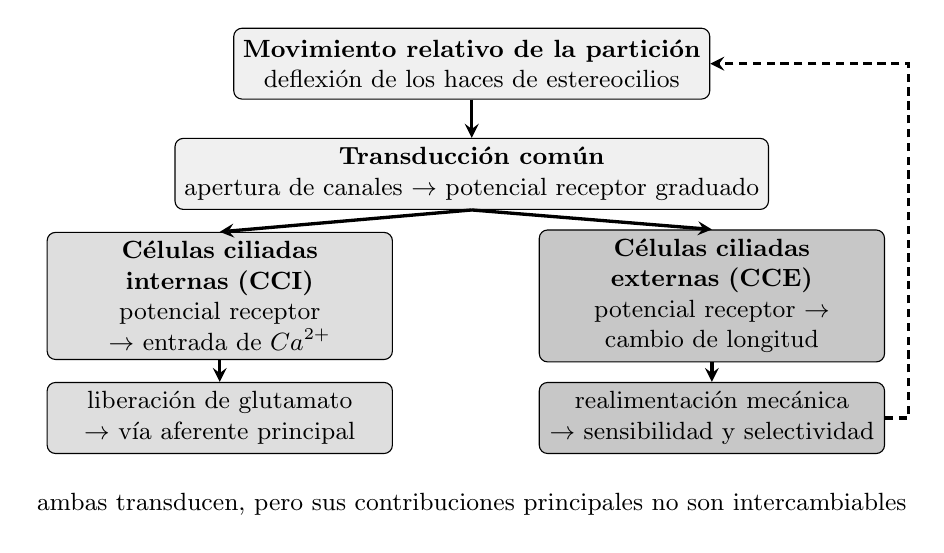
\begin{tikzpicture}[font=\small,>=stealth,x=1cm,y=1cm]
    \tikzset{
        common/.style={
            draw,rounded corners=3pt,fill=black!6,
            minimum width=4.30cm,minimum height=0.90cm,align=center
        },
        cci/.style={
            draw,rounded corners=3pt,fill=black!13,
            text width=4.15cm,minimum height=0.90cm,align=center
        },
        cce/.style={
            draw,rounded corners=3pt,fill=black!22,
            text width=4.15cm,minimum height=0.90cm,align=center
        },
        flow/.style={->,very thick}
    }

    \node[common] (motion) at (5.75,5.05)
        {\textbf{Movimiento relativo de la partición}\\
         deflexión de los haces de estereocilios};
    \node[common] (met) at (5.75,3.65)
        {\textbf{Transducción común}\\
         apertura de canales \(\rightarrow\) potencial receptor graduado};
    \draw[flow] (motion.south) -- (met.north);

    \node[cci] (ci) at (2.55,2.10)
        {\textbf{Células ciliadas internas (CCI)}\\
         potencial receptor \(\rightarrow\) entrada de \(\text{Ca}^{2+}\)};
    \node[cce] (ce) at (8.80,2.10)
        {\textbf{Células ciliadas externas (CCE)}\\
         potencial receptor \(\rightarrow\) cambio de longitud};
    \draw[flow] (met.south) -- (ci.north);
    \draw[flow] (met.south) -- (ce.north);

    \node[cci] (afferent) at (2.55,0.55)
        {liberación de glutamato\\
         \(\rightarrow\) vía aferente principal};
    \node[cce] (feedback) at (8.80,0.55)
        {realimentación mecánica\\
         \(\rightarrow\) sensibilidad y selectividad};
    \draw[flow] (ci.south) -- (afferent.north);
    \draw[flow] (ce.south) -- (feedback.north);

    \draw[->,very thick,densely dashed] (feedback.east) -- (11.30,0.55)
        -- (11.30,5.05) -- (motion.east);

    \node[align=center] at (5.75,-0.55)
        {ambas transducen, pero sus contribuciones principales no son
         intercambiables};
\end{tikzpicture}
